% Document
\documentclass[12pt, a4paper]{article}
\usepackage[T1]{fontenc}
\usepackage[utf8]{inputenc}
\usepackage{authblk}
\usepackage{lipsum}

% Figure and table formating
\usepackage{epsfig}
\usepackage{tabu}
\usepackage{rotating}
\usepackage{pbox}
\usepackage{framed, multicol}
\usepackage[framemethod=TikZ]{mdframed}
\usepackage{float}
\usepackage[left=1.25 in, right=1.25 in, top=1.25 in, bottom=1.25 in]{geometry}
\usepackage{csvsimple}

% Fonts - Mathtime
%\usepackage{txfonts}
\usepackage{amsmath} % Add amssymb if not using Mathtime

% Text
\setlength{\parindent}{0.5in}
\frenchspacing  \tolerance = 800  \hyphenpenalty = 800

\usepackage{lineno} % Line numbers
\def\linenumberfont{\normalfont\footnotesize\ttfamily}
\setlength\linenumbersep{0.2 in}

\usepackage{setspace}

% Format section and subsection headers
\makeatletter
\renewcommand{\section}{\@startsection
{section}%                   % the name
{1}%                         % the level
{0mm}%                       % the indent
{-\baselineskip}%            % the before skip
{0.5\baselineskip}%          % the after skip
{\normalfont\bf\large}} % the style

\renewcommand{\subsection}{\@startsection
{subsection}%                   % the name
{2}%                         % the level
{0mm}%                       % the indent
{-\baselineskip}%            % the before skip
{0.5\baselineskip}%          % the after skip
{\normalfont\bf}} % the style
\makeatother

% Other
\usepackage{graphicx}
\usepackage[singlelinecheck=false,font=small,labelfont=bf]{caption}

% Bibliography
\usepackage[numbers, compress]{natbib} % Bibliography - APA
\bibpunct{(}{)}{;}{a}{}{,}

% Format the Bibliography appropriately
% increase \bibhang to take care of the numbers
\setlength{\bibhang}{0pc}
\makeatletter
% patch \@lbibitem to print the current number before the authors
\patchcmd{\@lbibitem}
  {]}
  {] \theNAT@ctr. \newline }
  {}{}
\makeatother


%%%%%% FRONT MATTER %%%%%%%%%

\begin{document}

\linenumbers

\doublespacing

\noindent
\Large{\textbf{Supporting Information}}

\normalsize

\section*{Appendix 1: Implementation of the Crofton Method}

The algorithm for fitting the Crofton Method \citep{Crofton1971a} proceeds as follows. First, obtain a dataset
with $n$ hosts where each host has some parasite intensity 0 to $p_{max}$. Starting
with the full dataset, guess a vector of pre-mortality parameters $(N_p, \mu_p, k_p)$ and given
these parameters calculate the predicted number of hosts with $0, 1, 2, \dots
p_{max}$.  Compare the expected number of hosts with $0, 1, 2, \dots  p_{max}$ parasites
to the observed number hosts with $0, 1, 2, \dots p_{max}$ parasites and calculate
the $\chi^2$-squared statistic associated with your observed and predicted vectors. In reality, one often has to bin the parasite intensity data because all
parasite intensities are not represented in the dataset. Continue to guess $(N_p,
mu_p, k_p)$ vectors until a set of parameters is found that minimizes the $\chi^2$-
squared statistic.

Second, choose a truncation value ($t_1$) such that $t_1 <
p_{max}$. Truncate the data such that $\text{data}_\text{truncated} <= t$ and repeat the above
iterative procedure to calculate another set of parameters $(N_{p2}, \mu_{p2}, k_{p2})$
that minimizes the $\chi^2$-squared statistic on the truncated data. Choose a new
truncated value $t_2 < t_1$ and repeat the first two steps. Continue to truncated
the dataset until it only contains hosts with 0, 1, and 2 parasites (or 3 bins).
As the method attempts to estimate three parameters, at least 3 classes are
needed if all 3 parameters are to be identifiable \citep{Royce1990}.

We provide an implementation and unit tests of the Crofton Method Supplementary Information 3.  Figure \ref{fig:crof_test} visually shows the results of these unit tests.

\section*{Appendix 2: Additional Figure}

See Figures 1 - 6.

\section*{Appendix 3: Code and unit tests for estimating parasite-induced host mortality}

Python code, unit tests, and a help file for the Crofton Method, the Adjei Method and the Likelihood Method can be found in \verb*#pihm_methods.py#, \verb*#test_pihm_methods.py#, and \verb*#help_file.txt#, respectively.

% These can be in the supplementary in later drafts!

\begin{figure}

    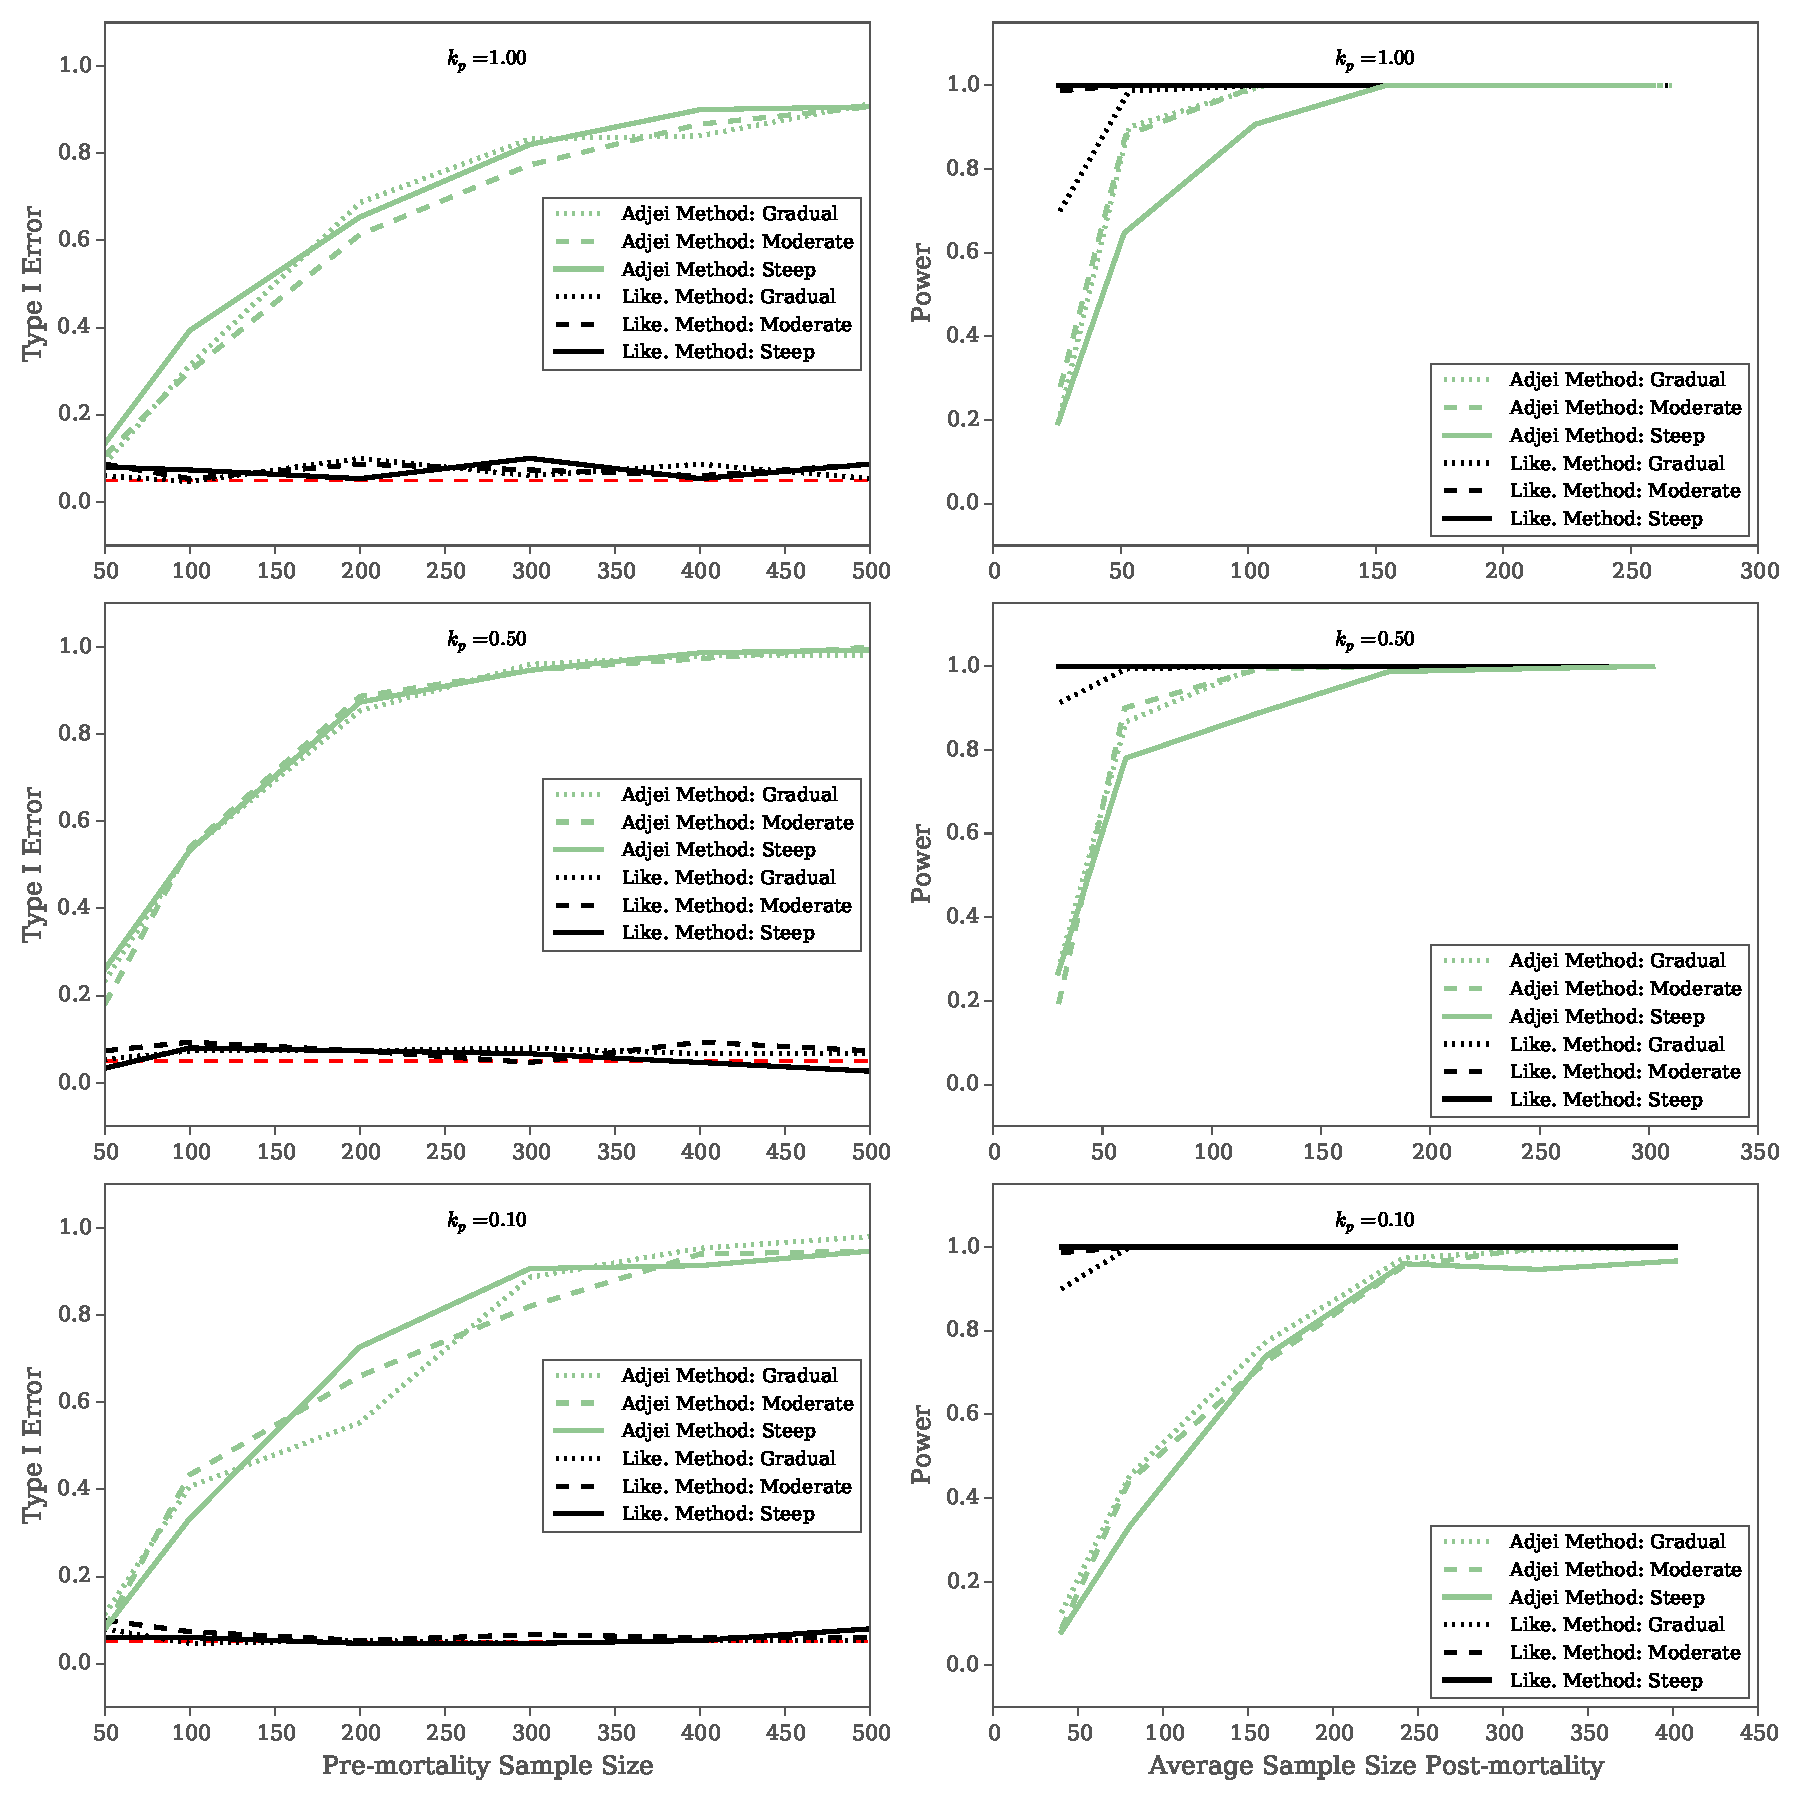
\includegraphics[width=\textwidth]{/Users/mqwilber/Repos/parasite_mortality/results/typeIpower_figure_for_mu50}

    \caption{The type I error rate and the power of the Likelihood Method (solid line) and the Adjei Method (dashed lines) when $\mu_p = 50$ for various shapes of the host survival function and levels of aggregation $k_p$.  The first column gives the type I error rate of each method for falsely detecting PIHM when none is present.  The red line gives the the pre-set type I error rate of $\alpha = 0.05$.  The second column gives the power of a given method to detect PIHM when it is actually occurring. }
    \label{fig:typeI50}

\end{figure}

\begin{figure}

    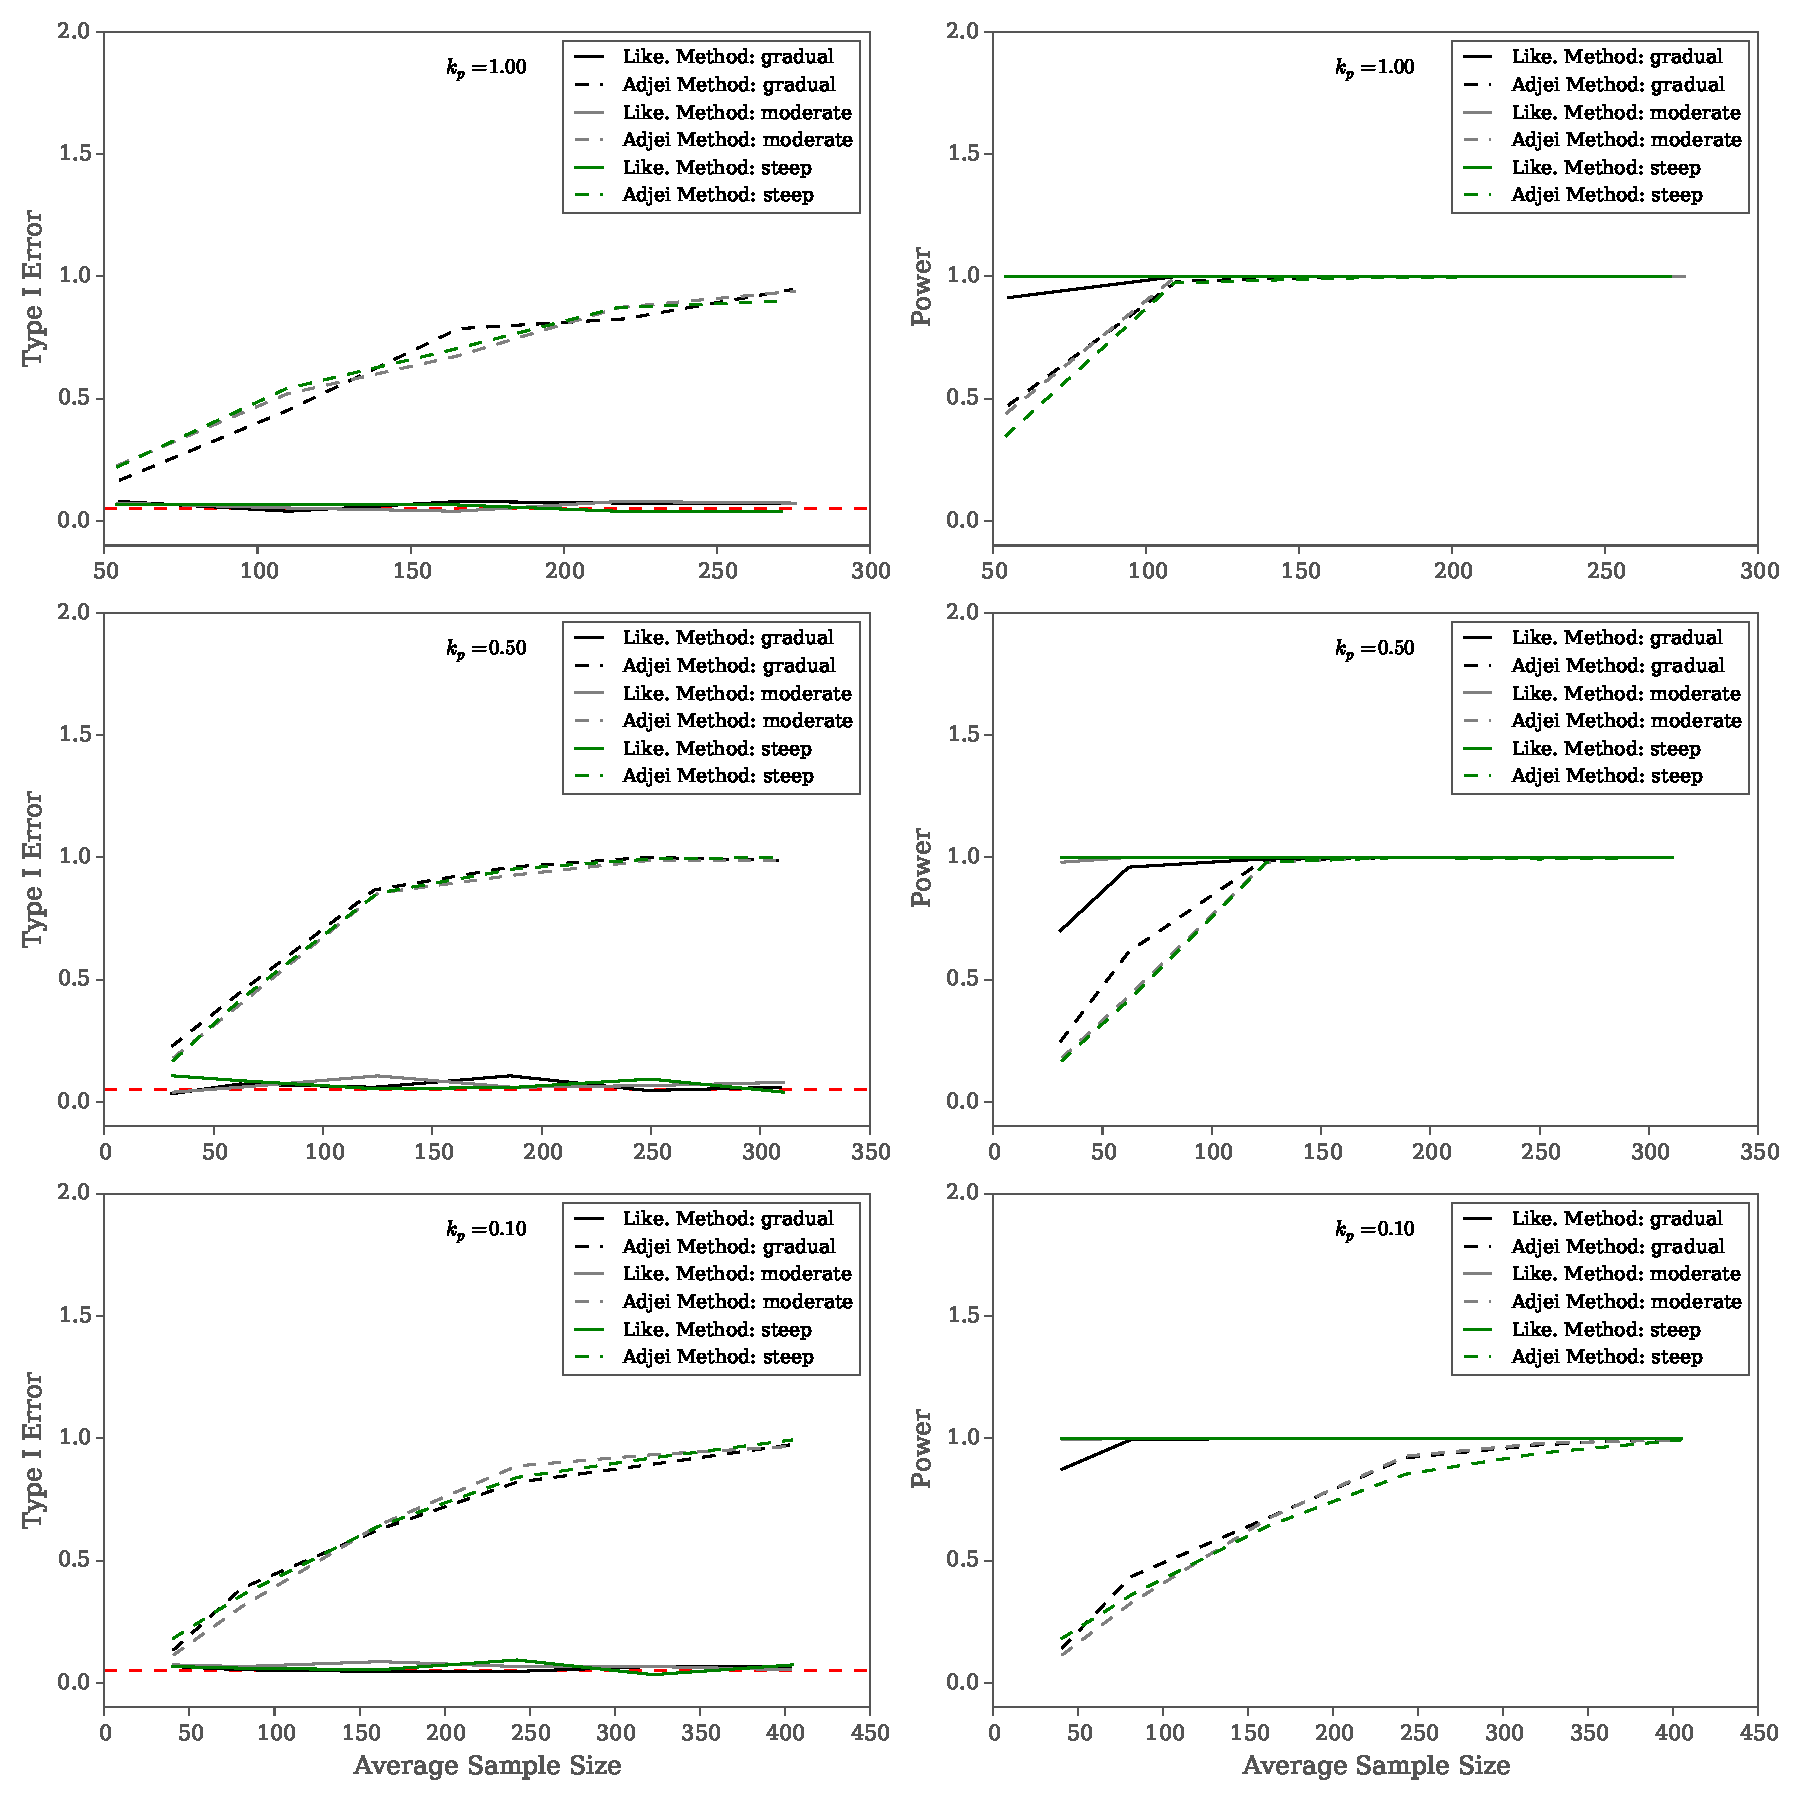
\includegraphics[width=\textwidth]{/Users/mqwilber/Repos/parasite_mortality/results/typeIpower_figure_for_mu100}

    \caption{The type I error rate and the power of the Likelihood Method (solid line) and the Adjei Method (dashed lines) when $\mu_p = 100$ for various shapes of the host survival function and levels of aggregation $k_p$.  The first column gives the type I error rate of each method for falsely detecting PIHM when none is present.  The red line gives the the pre-set type I error rate of $\alpha = 0.05$.  The second column gives the power of a given method to detect PIHM when it is actually occurring. }
    \label{fig:typeI100}

\end{figure}

\begin{figure}

    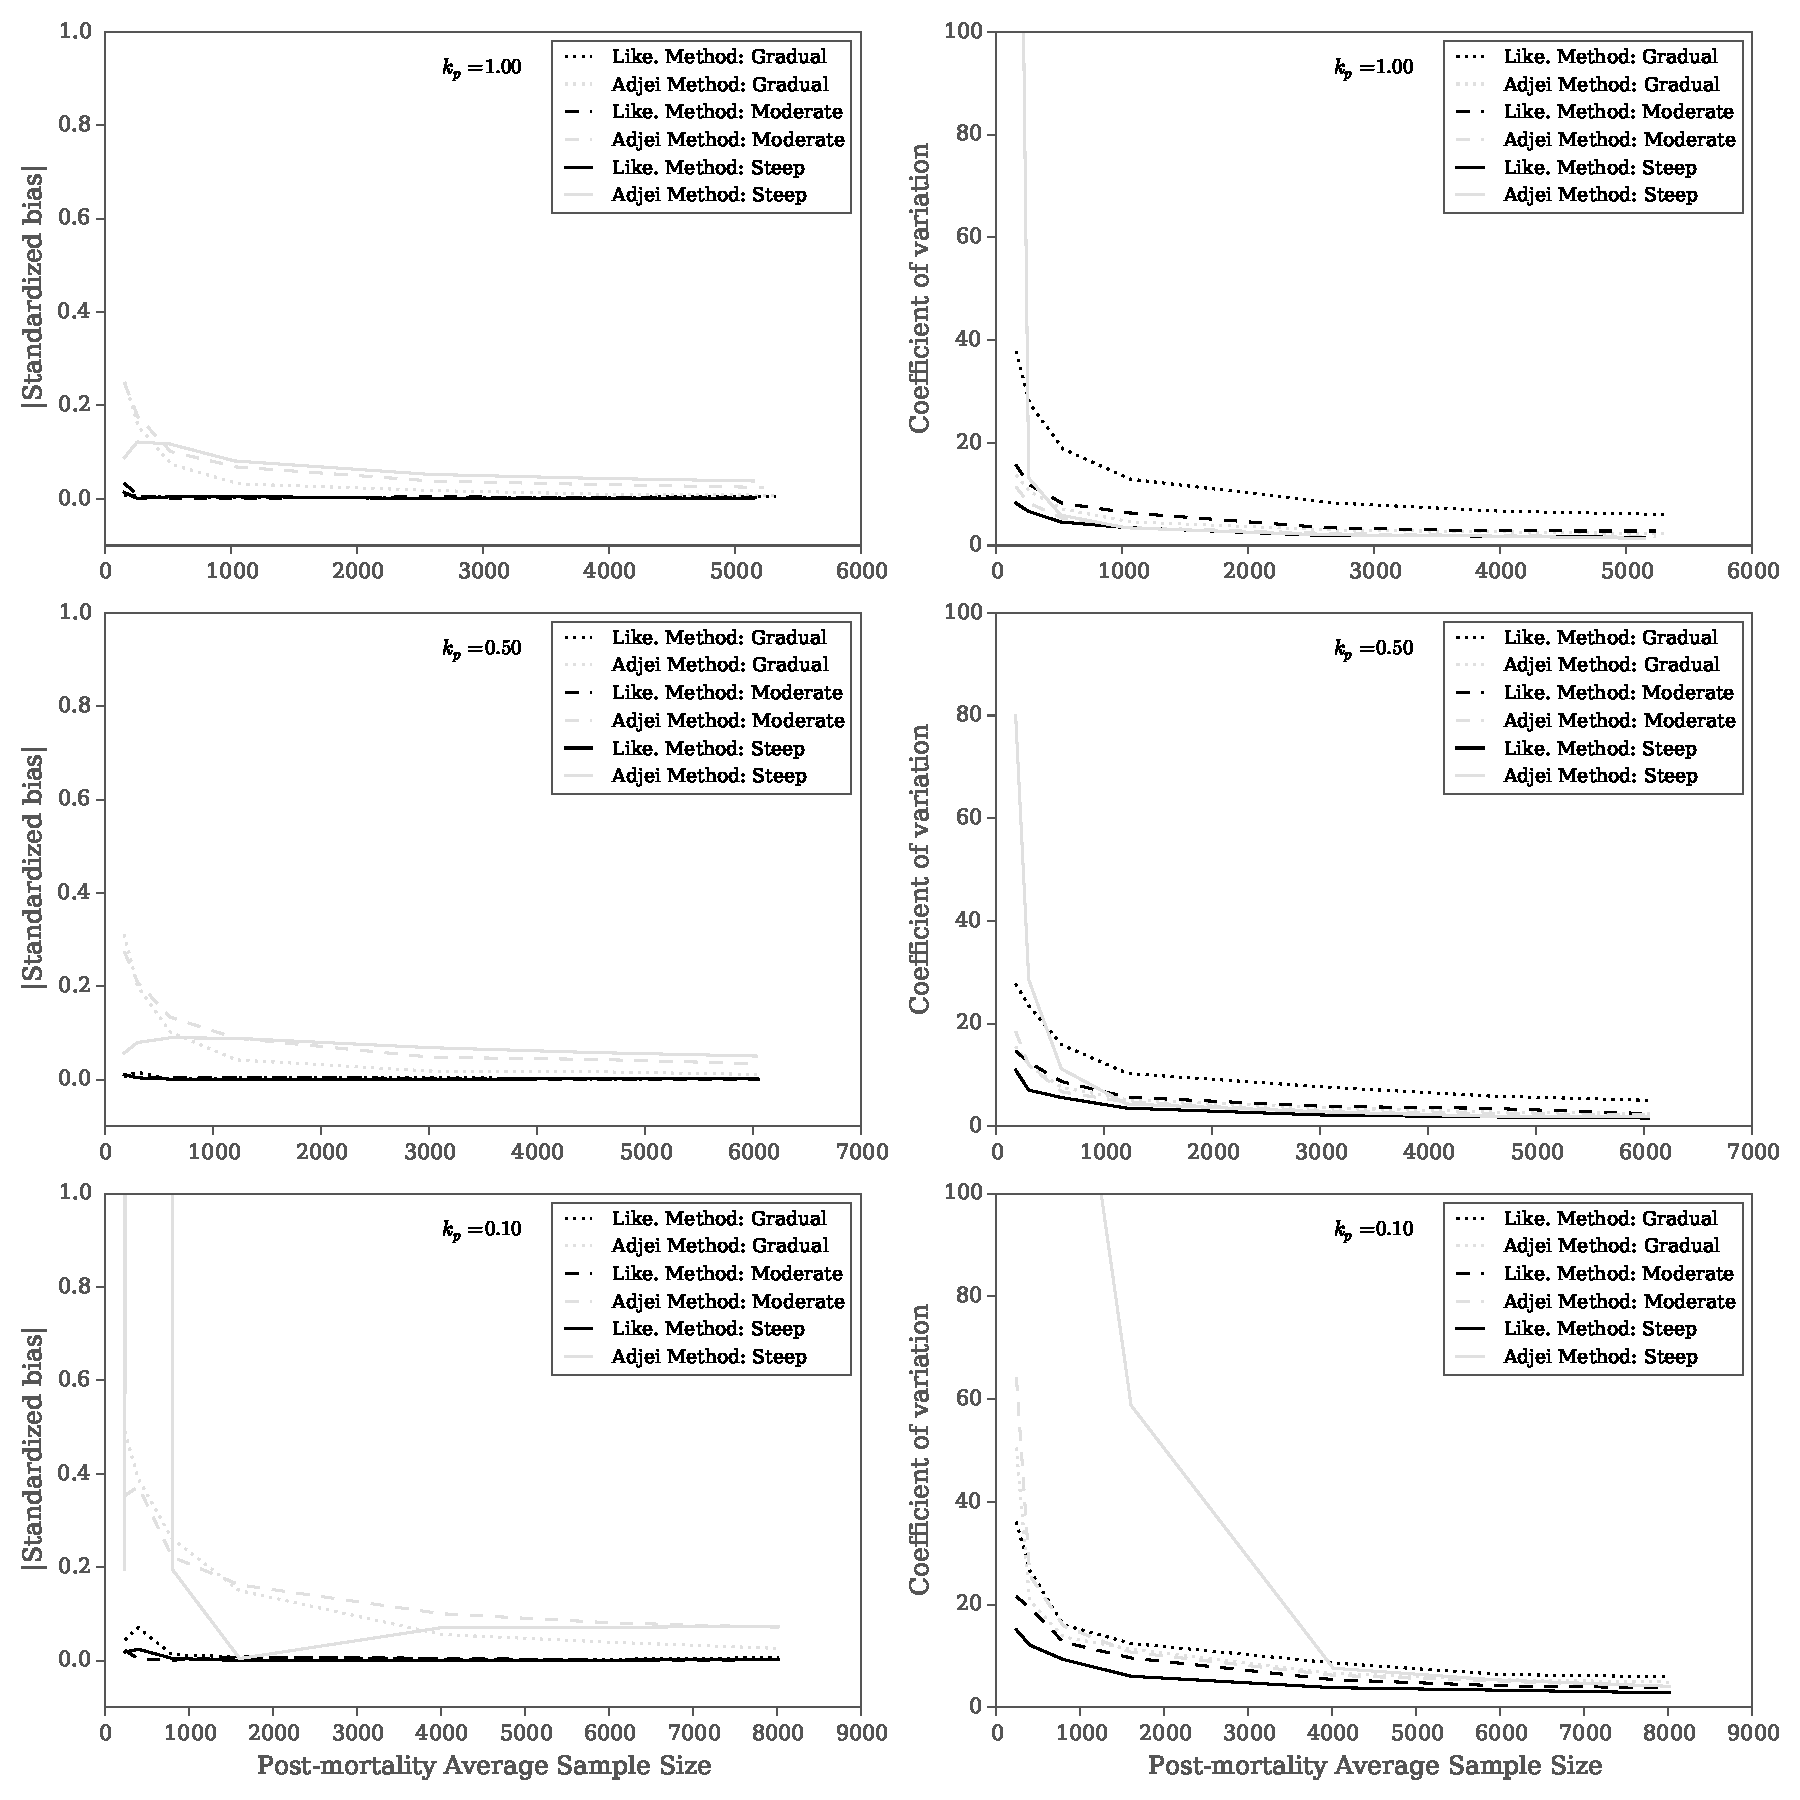
\includegraphics[width=\textwidth]{/Users/mqwilber/Repos/parasite_mortality/results/bais_prec_figure_for_ld50_mu50}

    \caption{The bias and the precision of the Likelihood Method (solid line) and the Adjei Method (dashed lines) when $\mu_p = 50$ for various shapes of the host survival function and levels of aggregation $k_p$ when estimating $LD_{50}$.  The first column gives the bias of each method's $LD_{50}$ estimate over 150 simulations. The second column gives the precision of each method's $LD_{50}$ estimate over 150 simulations.}

    \label{fig:biasld50_50}

\end{figure}

\begin{figure}

    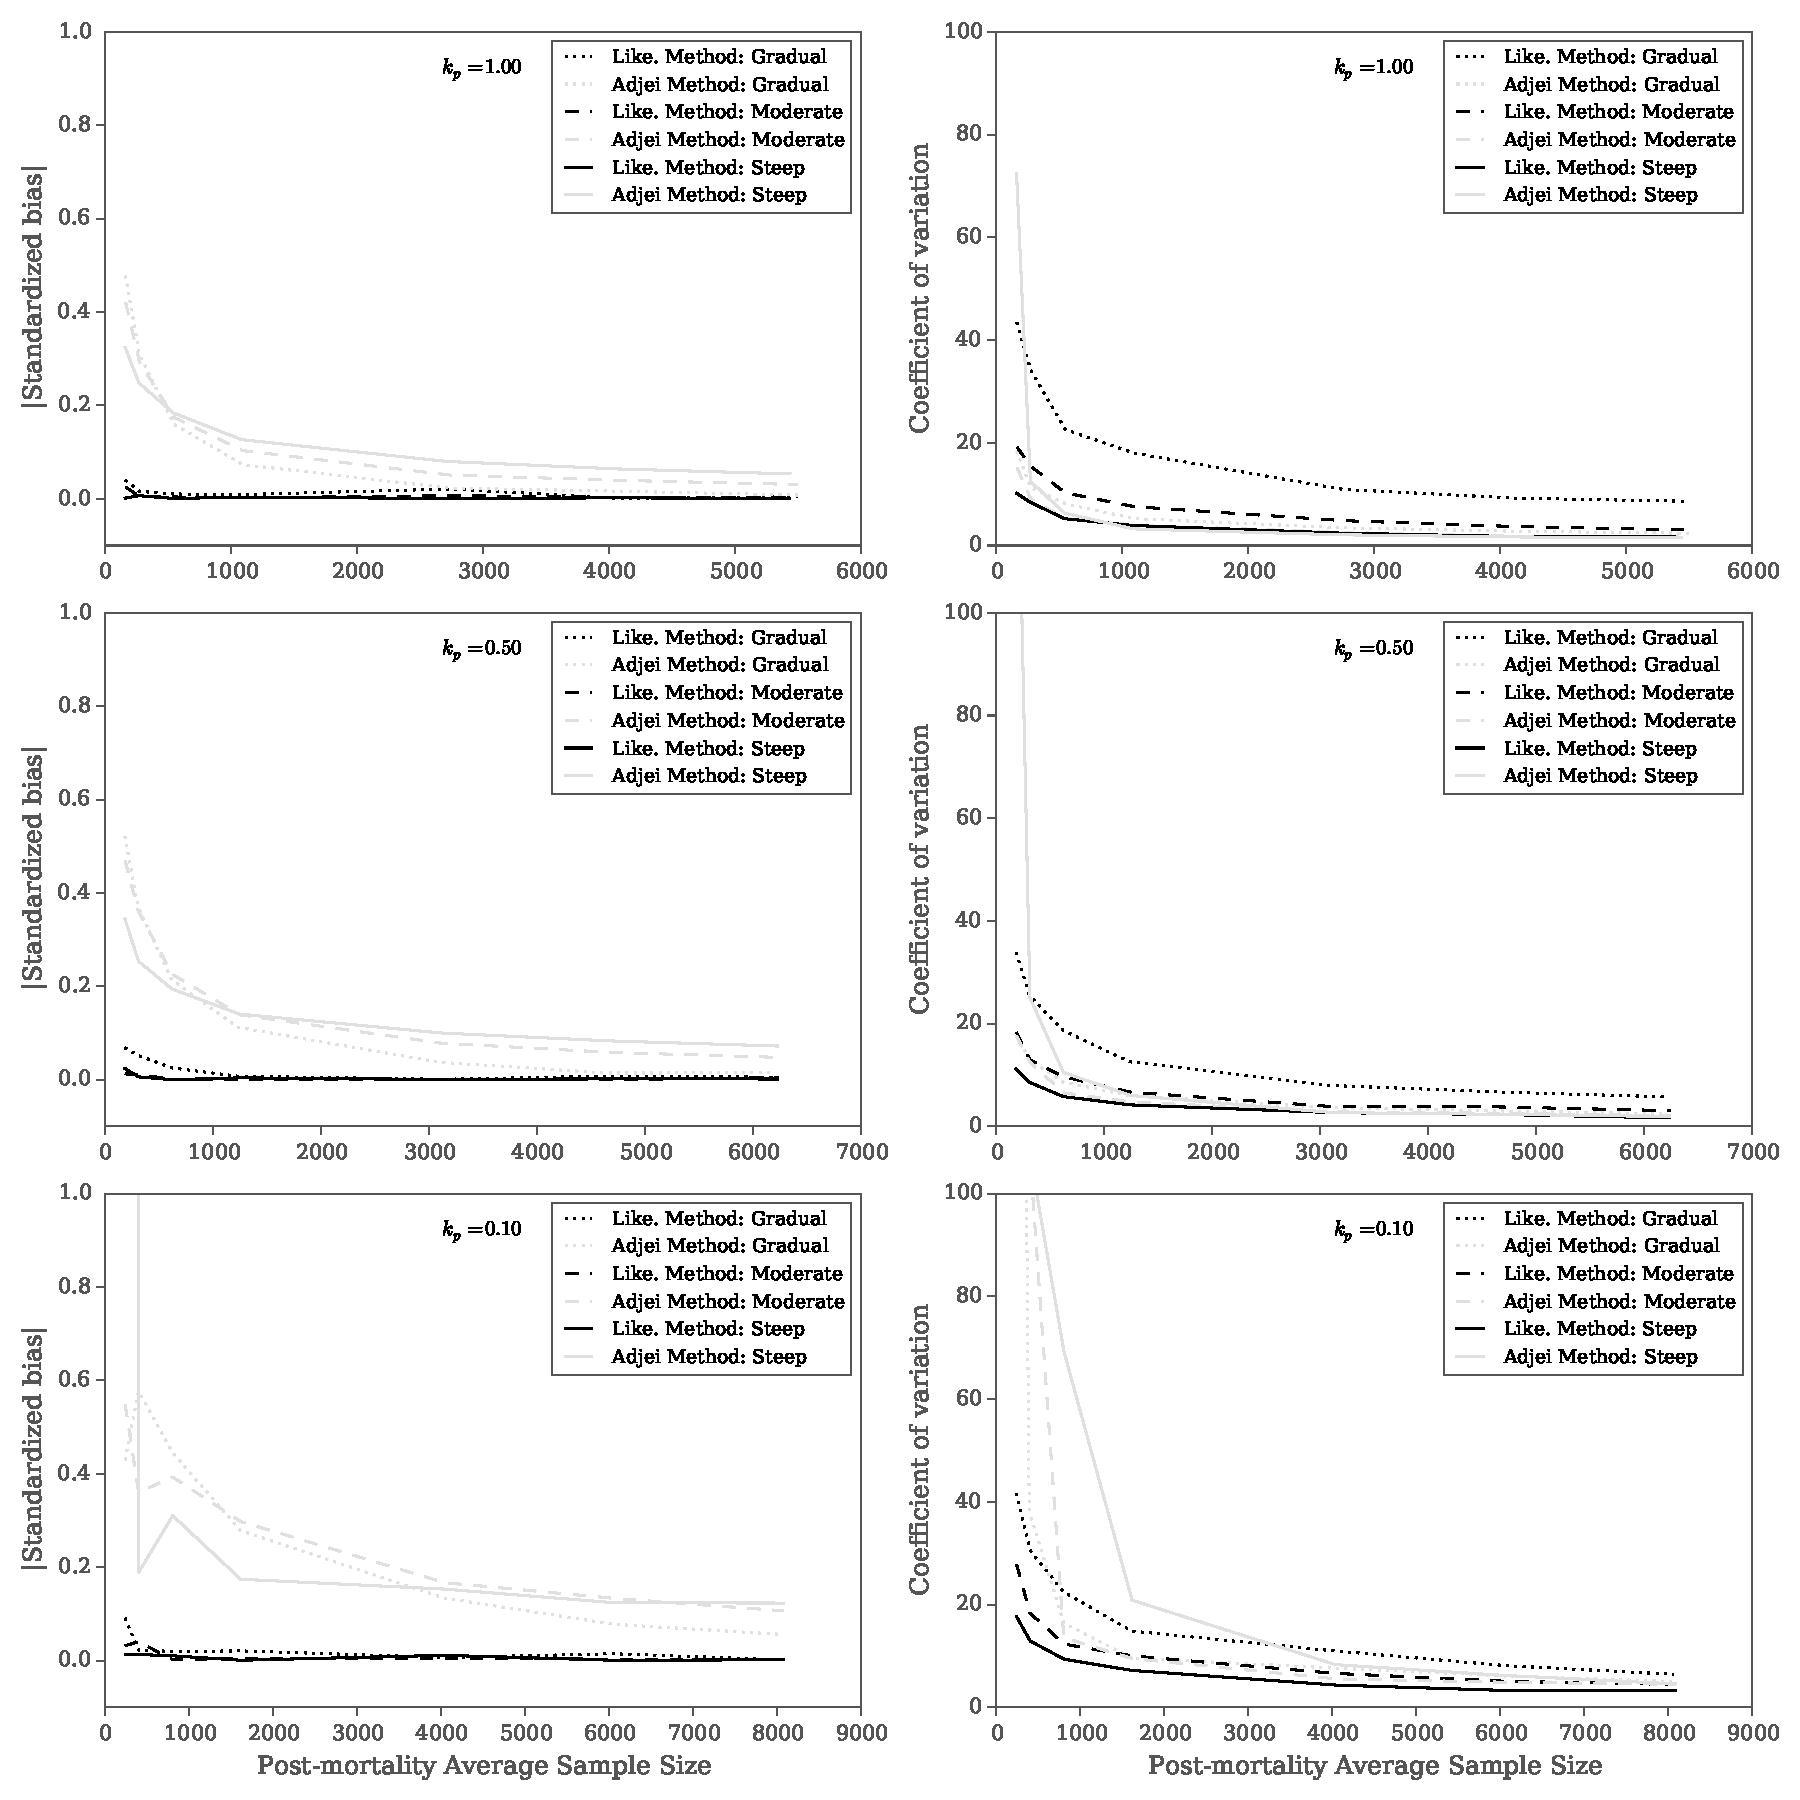
\includegraphics[width=\textwidth]{/Users/mqwilber/Repos/parasite_mortality/results/bais_prec_figure_for_ld50_mu100}

    \caption{The bias and the precision of the Likelihood Method (solid line) and the Adjei Method (dashed lines) when $\mu_p = 100$ for various shapes of the host survival function and levels of aggregation $k_p$ when estimating $LD_{50}$.  The first column gives the bias of each method's $LD_{50}$ estimate over 150 simulations. The second column gives the precision of each method's $LD_{50}$ estimate over 150 simulations.}

    \label{fig:biasld50_100}

\end{figure}

\begin{figure}

    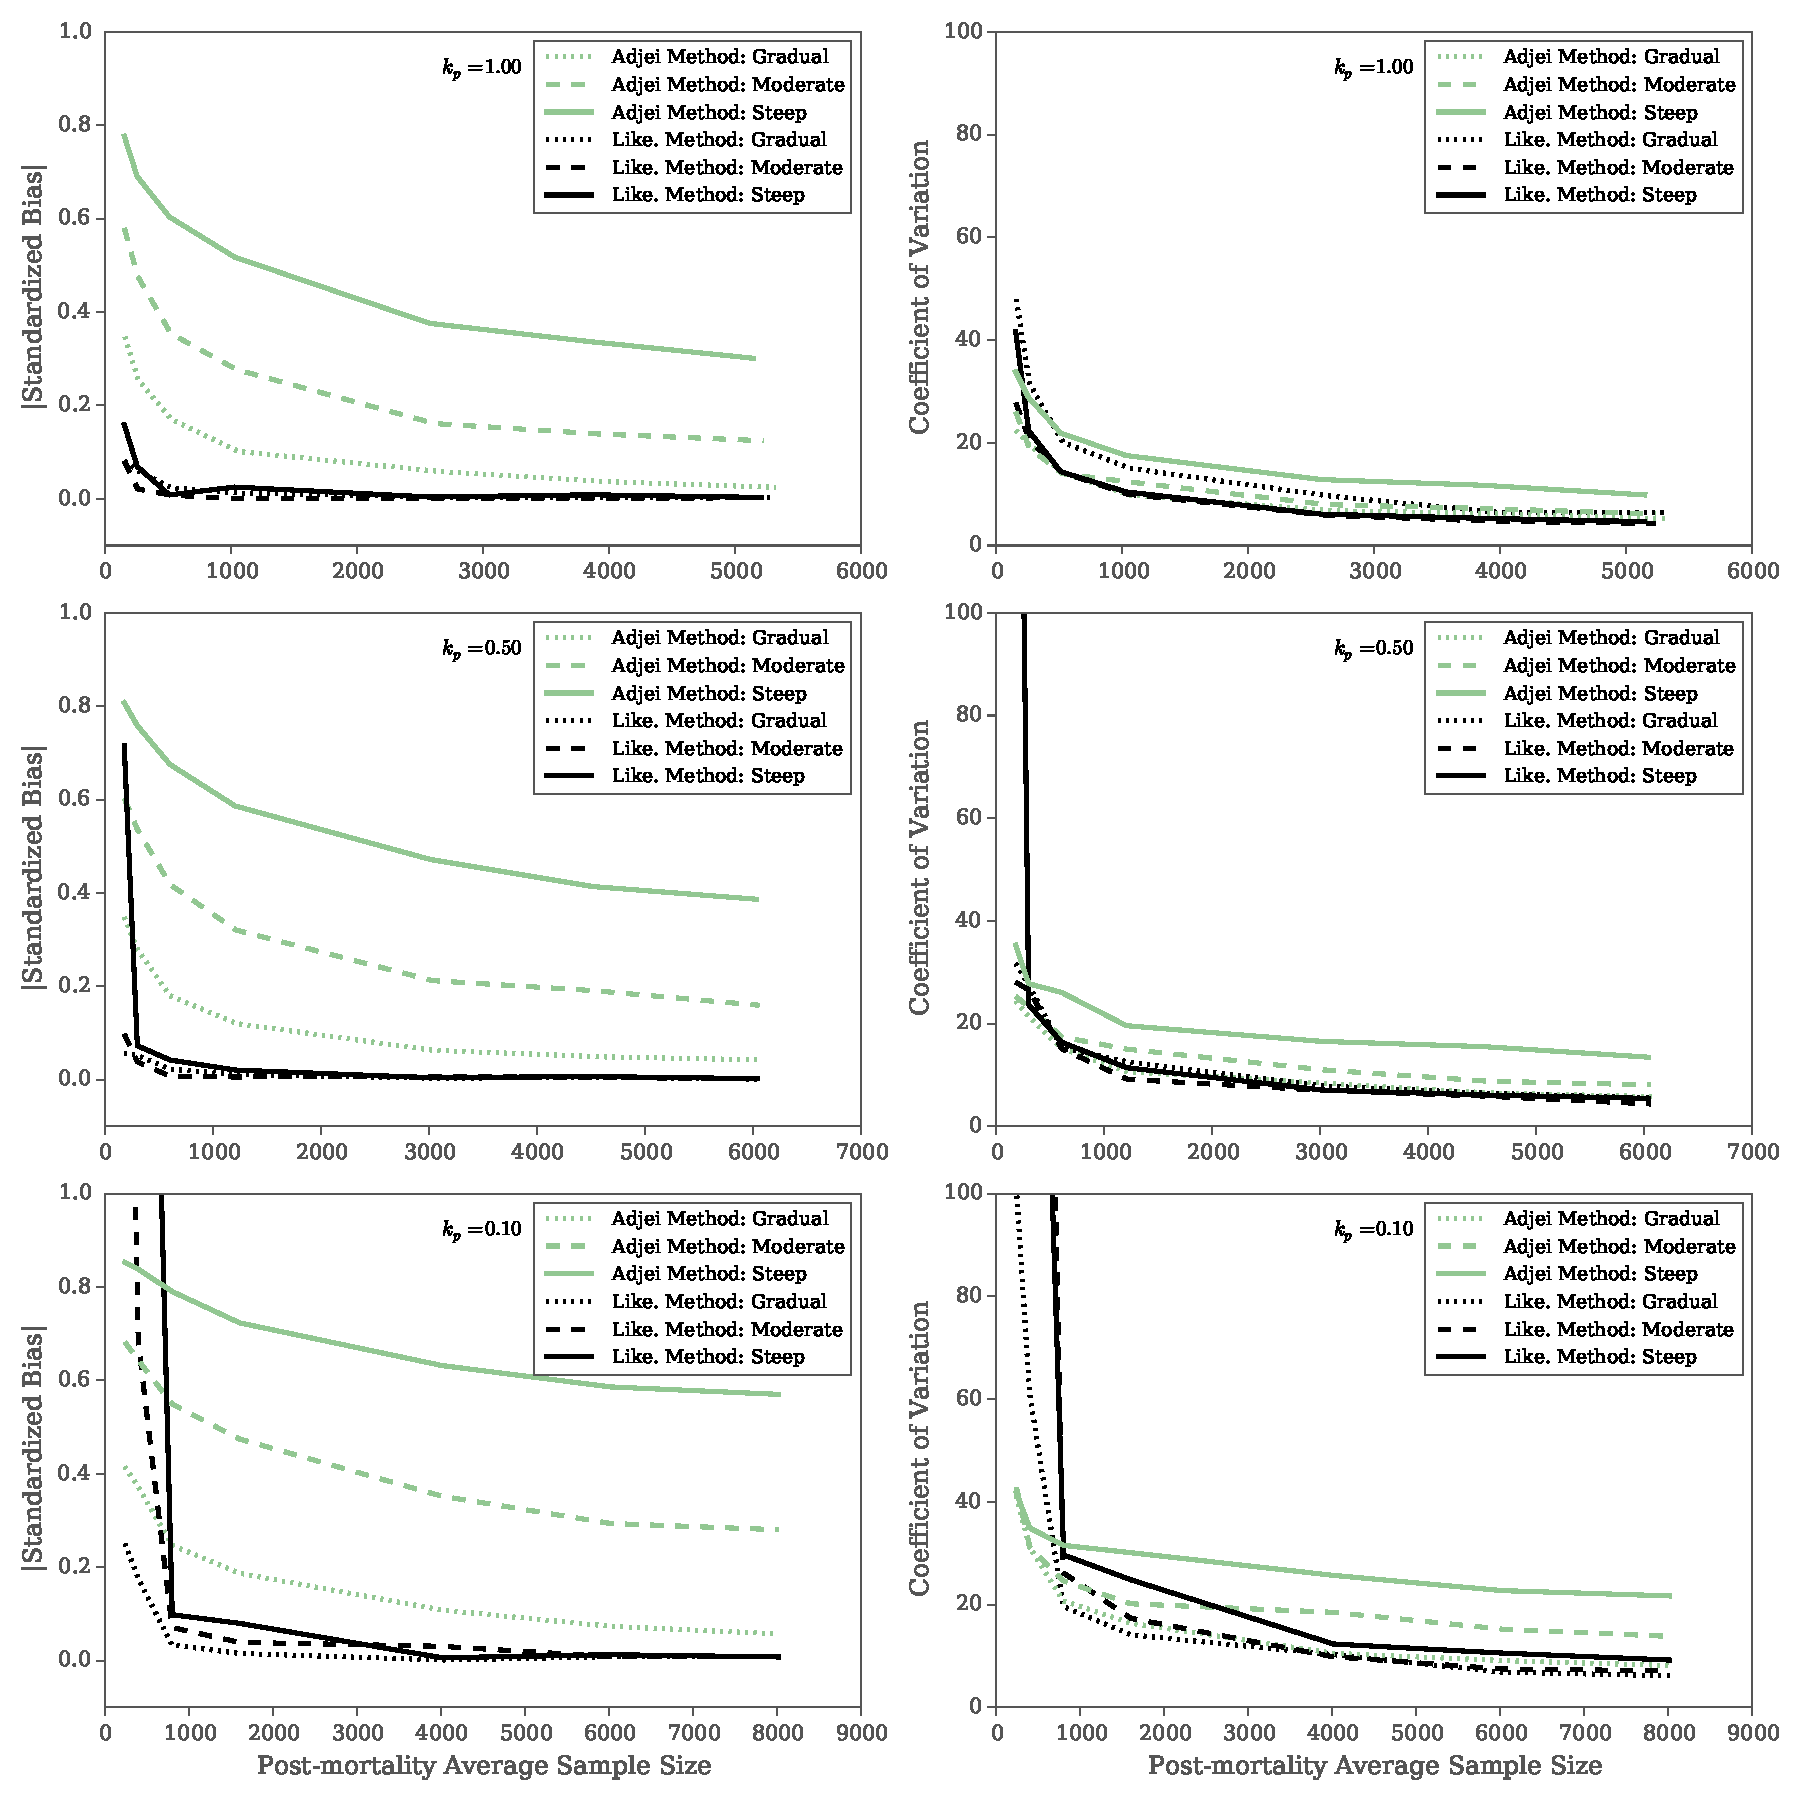
\includegraphics[width=\textwidth]{/Users/mqwilber/Repos/parasite_mortality/results/bais_prec_figure_for_a_mu50}

    \caption{The bias and the precision of the Likelihood Method (solid line) and the Adjei Method (dashed lines) when $\mu_p = 50$ for various shapes of the host survival function and levels of aggregation $k_p$ when estimating the $a$ parameter of the host survival function.  The first column gives the bias of each method's $a$ estimate over 150 simulations. The second column gives the precision of each method's $a$ estimate over 150 simulations.}

    \label{fig:biasa_50}

\end{figure}

\begin{figure}

    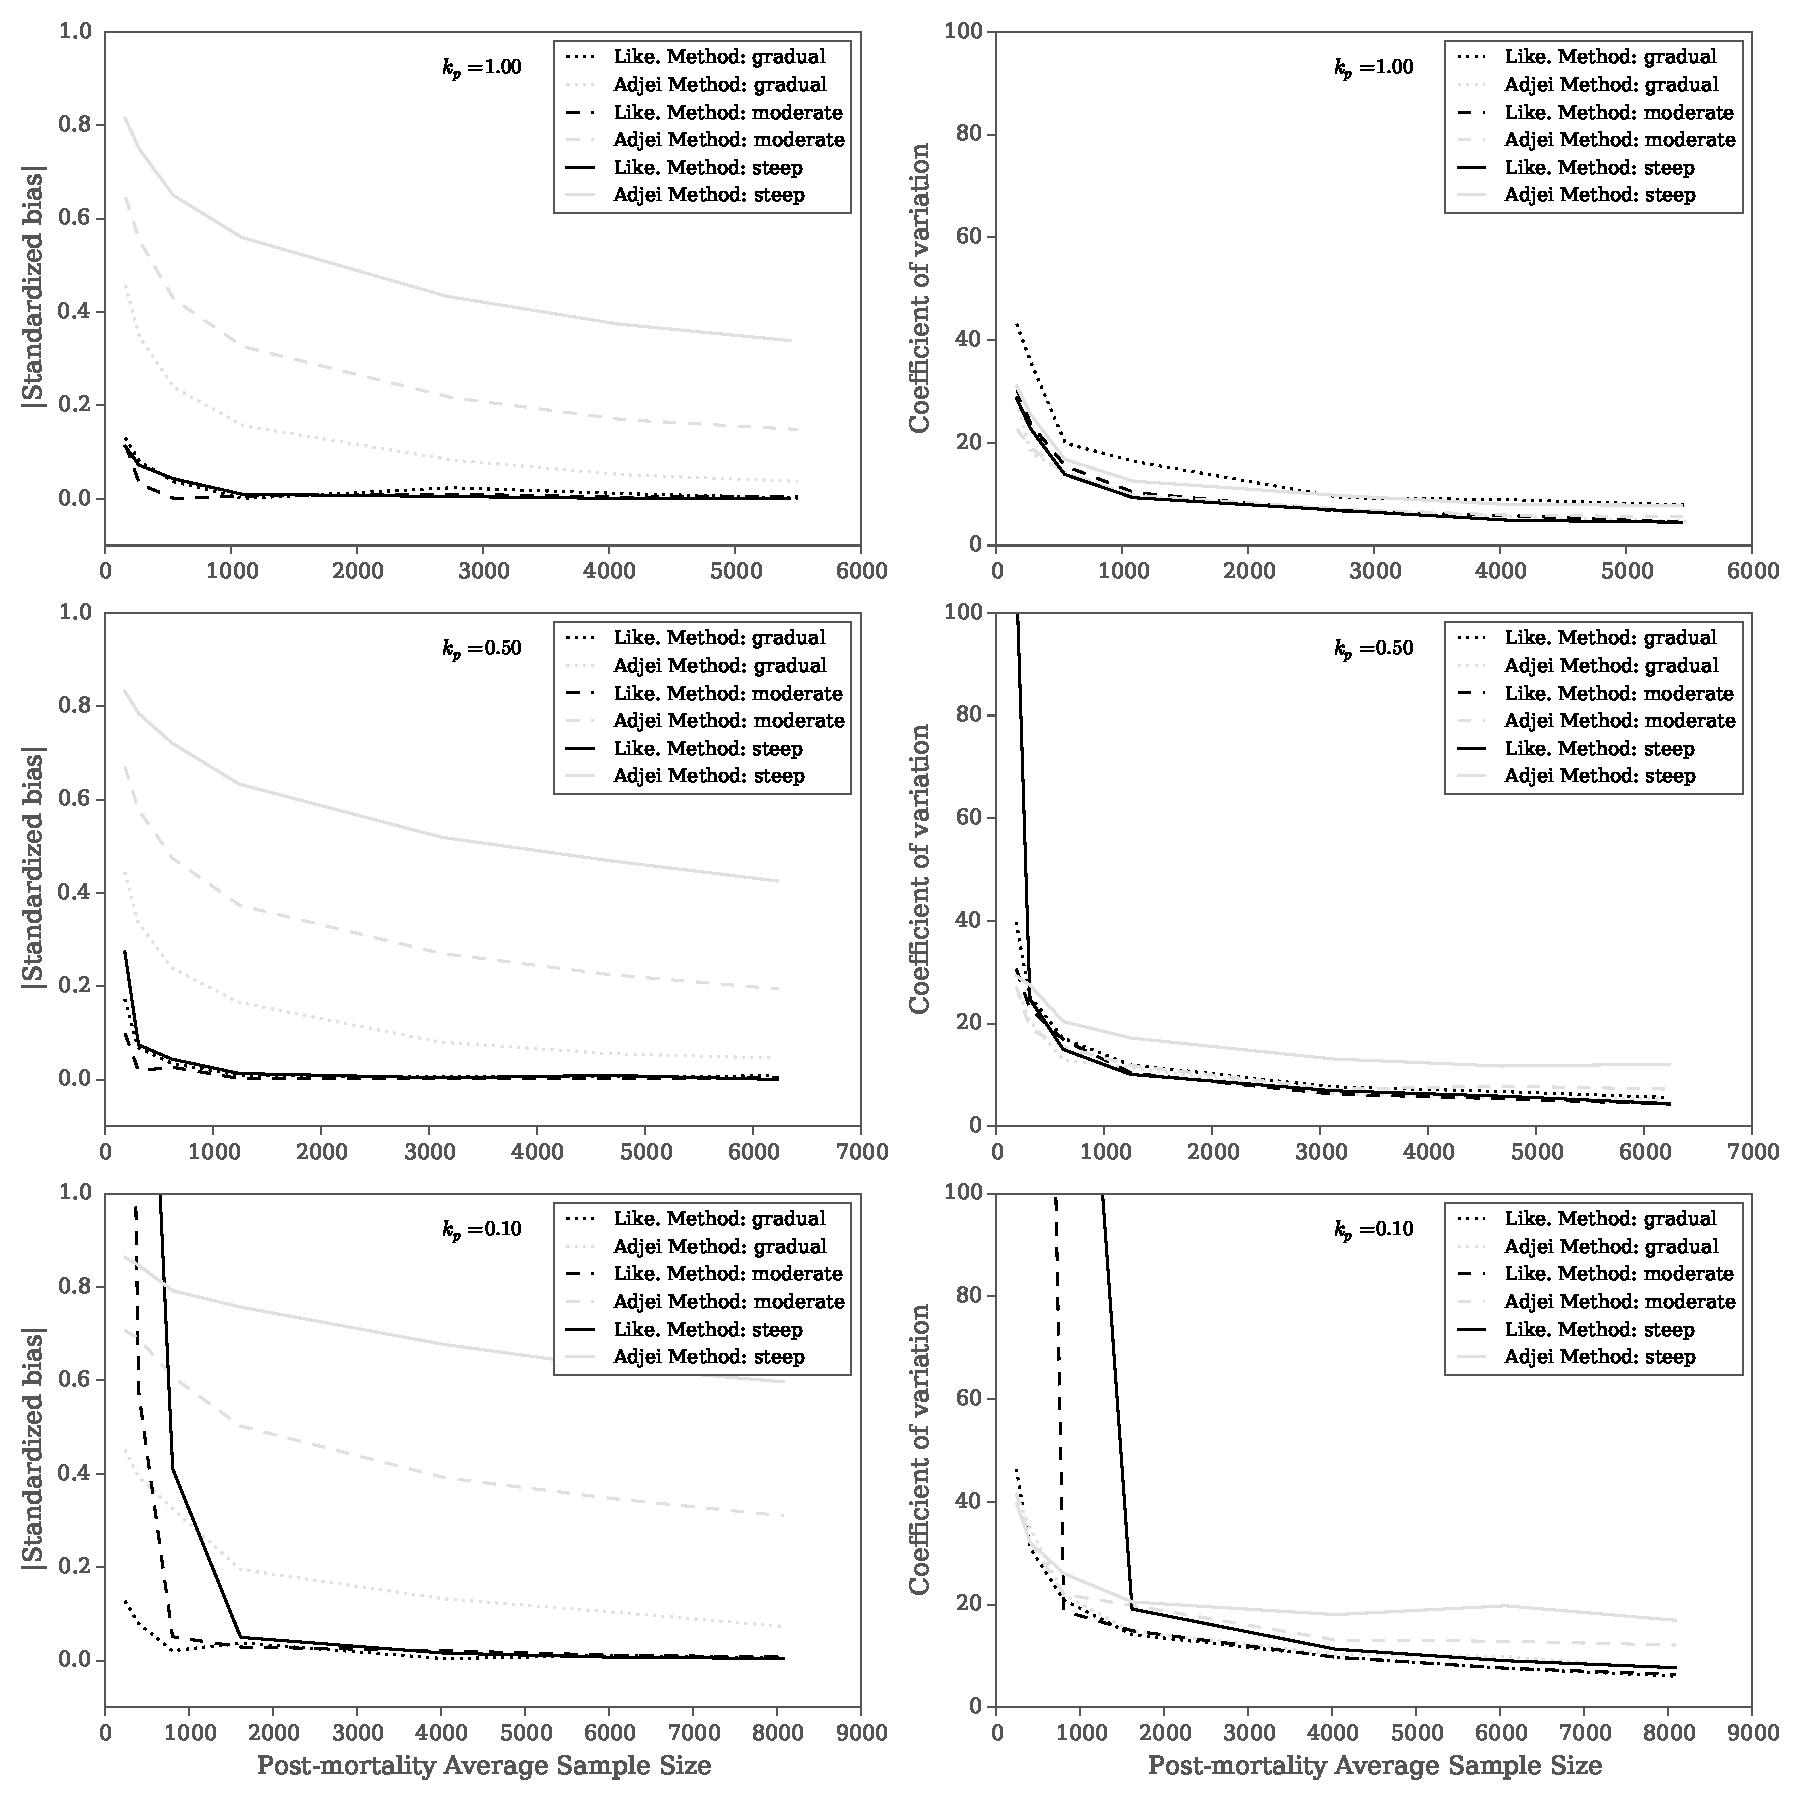
\includegraphics[width=\textwidth]{/Users/mqwilber/Repos/parasite_mortality/results/bais_prec_figure_for_a_mu100}

    \caption{The bias and the precision of the Likelihood Method (solid line) and the Adjei Method (dashed lines) when $\mu_p = 100$ for various shapes of the host survival function and levels of aggregation $k_p$ when estimating the $a$ parameter of the host survival function.  The first column gives the bias of each method's $a$ estimate over 150 simulations. The second column gives the precision of each method's $a$ estimate over 150 simulations.}

    \label{fig:biasa_100}

\end{figure}

\begin{figure}
    \centering
    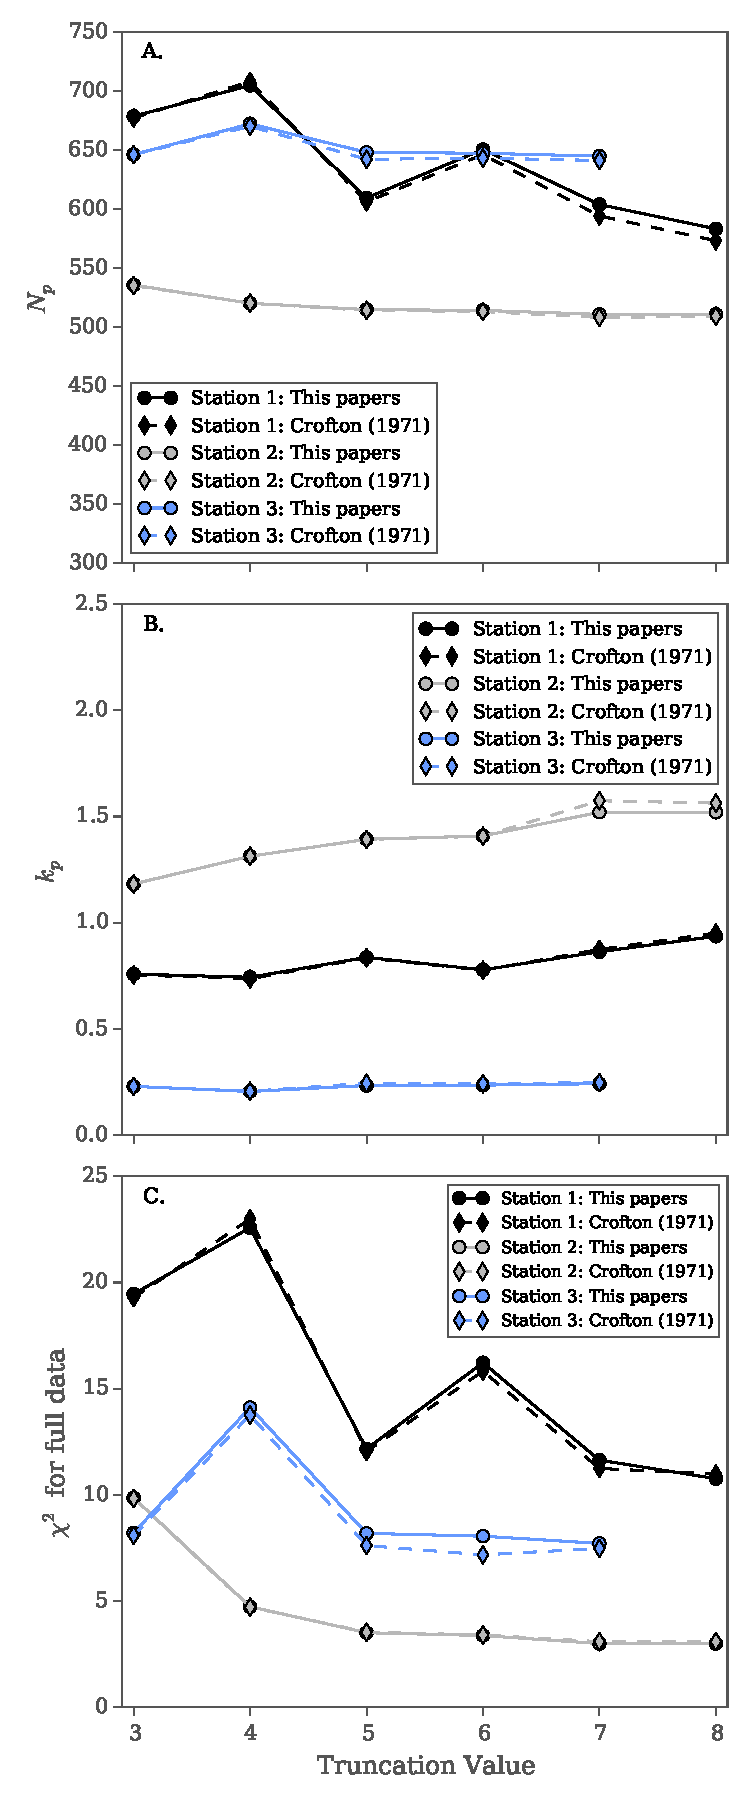
\includegraphics[width=0.5\textwidth]{/Users/mqwilber/Repos/parasite_mortality/results/compare_crofton.pdf}
    \caption{A comparison of this papers implementation of the Crofton Method with the results given in \cite{Crofton1971a}.  Three of the 6 stations fit by \cite{Crofton1971a} are shown here and all three show that the two implementations give very similar results.}
    \label{fig:crof_test}

\end{figure}



\singlespacing
\bibliographystyle{/Users/mqwilber/Dropbox/Documents/Bibformats/ecology_letters.bst}
\bibliography{/Users/mqwilber/Dropbox/Documents/Bibfiles/Projects_and_Permits-parasite_host_mortality}

\end{document}

